\chapter{Simulation with Vectors}

In an earlier chapter, you wrote a python program that simulated the flight of a hammer to predict its altitude. Your simulation
dealt only with scalars.  Now, you are ready to create simulations of positions, velocities, accelerations, and forces as vectors.

In this chapter, you are going to simulate two moons that, as they wandered through the vast universe,  get caught
in each other's gravity well.   We will assume there are no other forces acting upon the moons.

\section{Force, Acceleration, Velocity, and Position}
\index{gravitation}
We talked about the magnitude of a gravitational attraction between two masses:

$$F = G\frac{m_1 m_2}{r^2}$$

where $F$ is the magnitude of the force in newtons, $m_1$ and $m_2$ are the masses in kg,  $r$ is the distance between them in meters, and $g$ is the universal gravitational constant: $6.67430 \times 10^{−11}$.

What is the direction?  For the two moons,  the force on moon 1 will pull toward moon 2.  
Likewise, the force on moon 2 will pull toward moon 1.
 
Of course,  if something is big (like the sun),  you need to be more specific:  The force points directly at the center
of mass of the object that is generating the force.

Each of the moons will start off with a velocity vector. That velocity vector will change over time as the moon is
accelerated by the force of gravity.  If you have a mass $m$ with an initial velocity vector of $\vec{v_0}$ that is being accelerated with a constant force vector $\vec{F}$, at time $t$, the new velocity vector will be:

$$\vec{v}_t = \vec{v}_0  + \frac{t}{m}  \vec{F}$$

If an object is at an initial position vector of $\vec{p_0}$ and moves with a constant velocity vector $\vec{v}$ 
for time $t$,  the new position will be given by 

$$\vec{p}_t = \vec{p}_0  + t \vec{v}$$

\section{Simulations and Step Size}

As two moons orbit each other,  the force, acceleration, velocity, and position are changing smoothly and continuously.  It is difficult to simulate truly continuous things on a digital computer.

However,  think about how a movie shows you many frames each second.   Each frame is a still picture of the 
state of the system.  The more frames per second,  the smoother it looks.

We do a similar trick in simulations. We say "We are going run our simulation in 2 hour steps. We will assume
that the acceleration and velocity were constant for those two hours.   We will update our position vectors accordingly, then we will recalculate our acceleration and velocity vectors."

Generally, as you make the step size smaller,  your simulation will get more accurate and take longer to execute.

\section{Make a Text-based Simulation}

To start, you are going to write a Python program that simulates the moons and prints out their
position for every time step.  Later, we will add graphs and even animation.

We are going to assume the two moons are traveling the same plane so we can do all the math and graphing 
in 2 dimensions.

Each moon will be represented by a dictionary containing the state of the moon:
\begin{itemize}
\item Its mass in kilograms
\item Its position --- A 2-dimensional vector represent $x$ and $y$ coordinates of the center of the moon.
\item Its velocity --- A 2-dimensional vector
\item Its radius --- Each moon has a radius so we know when the centers of the two moons are so close to each other that they must have collided.
\item Its color --- We will use that when do the plots and animations.  One moon will be red, the other blue.
\end{itemize}

There will then be a loop where we will update the positions of the moons and then recalculate the 
acceleration and velocities.    

How much time will be simulated?  100 days or until the moons collide,  whichever
comes first.

We will use numpy arrays to represent our vectors.

Create a file called \filename{moons.py}, and type in this code:

\begin{verbatim}
import numpy as np

# Constants
G = 6.67430e-11              # Gravitational constant (Nm^2/kg^2)
SEC_PER_DAY = 24 * 60 * 60   # How many seconds in a day?
MAX_TIME = 100 * SEC_PER_DAY # 100 days
TIME_STEP = 2 * 60 * 60      # Update every two hours

# Create the inital state of Moon 1
m1 = {
    "mass": 6.0e22,  # kg
    "position": np.array([0.0, 200_000_000]),  # m
    "velocity": np.array([100.0, 25.0]),  # m/s
    "radius": 1_500_000.0,  # m
    "color": "red" # For plotting
}

# Create the inital state of Moon 2
m2 = {
    "mass": 11.0e22,  # kg
    "position": np.array([0.0, -150_000_000]),  # m
    "velocity": np.array([-45.0, 2.0]),  # m/s
    "radius": 2_000_000.0,  # m
    "color": "blue" # For plotting
}  

# Lists to hold positions and time
position1_log = []
position2_log = []
time_log = []

# Start at time zero seconds
current_time = 0.0

# Loop until current time exceed Max Time
while current_time <= MAX_TIME:

    # Add time and positions to log
    time_log.append(current_time)
    position1_log.append(m1["position"])
    position2_log.append(m2["position"])
    
    # Print the current time and positions
    print(f"Day {current_time/SEC_PER_DAY:.2f}:")
    print(f"\tMoon 1:({m1['position'][0]:,.1f},{m1['position'][1]:,.1f})")
    print(f"\tMoon 2:({m2['position'][0]:,.1f},{m2['position'][1]:,.1f})")

    # Update the positions based on the current velocities
    m1["position"] = m1["position"] + m1["velocity"] * TIME_STEP
    m2["position"] = m2["position"] + m2["velocity"] * TIME_STEP

    # Find the vector from moon1 to moon2
    delta = m2["position"] - m1["position"]

    # What is the distance between the moons?
    distance = np.linalg.norm(delta)

    # Have the moons collided?
    if distance < m1["radius"] + m2["radius"]:
        print(f"*** Collided {current_time:.1f} seconds in!")
        break

    # What is a unit vector that points from moon1 toward moon2?
    direction = delta / distance

    # Calculate the magnitude of the gravitational attraction
    magnitude = G * m1["mass"] * m2["mass"] / (distance**2)

    # Acceleration vector of moon1 (a = f/m)
    acceleration1 = direction * magnitude / m1["mass"]

    # Acceleration vector of moon2
    acceleration2 = (-1 * direction) * magnitude / m2["mass"]

    # Update the velocity vectors
    m1["velocity"] = m1["velocity"] + acceleration1 * TIME_STEP
    m2["velocity"] = m2["velocity"] + acceleration2 * TIME_STEP

    # Update the clock
    current_time += TIME_STEP

print(f"Generated {len(position1_log)} data points.")
\end{verbatim}

When your run the simulation,  you will see the positions of the moons for 100 days:
\begin{verbatim}
> python3 moons.py 
Day 0.00:
	Moon 1:(0.0,200,000,000.0)
	Moon 2:(0.0,-150,000,000.0)
Day 0.08:
	Moon 1:(720,000.0,200,180,000.0)
	Moon 2:(-324,000.0,-149,985,600.0)
Day 0.17:
	Moon 1:(1,439,990.7,200,356,896.1)
	Moon 2:(-647,995.0,-149,969,507.0)
...
Day 100.00:
	Moon 1:(119,312,305.5,283,265,313.5)
	Moon 2:(17,393,287.9,-60,319,261.9)
Generated 1201 data points.
\end{verbatim}

Look over the code. Make sure you understand what every line does.

\section{Graph the Paths of the Moons}

Now, you will use the matplotlib to graph the paths of the moons. Add this line to the beginning of 
\filename{moons.py}.

\begin{verbatim}
import matplotlib.pyplot as plt
\end{verbatim}


Add this code to the end of your \filename{moons.py}:

\begin{verbatim}
# Convert lists to np.arrays
positions1 = np.array(position1_log)
positions2 = np.array(position2_log)

# Create a figure with a set of axes
fig, ax = plt.subplots(1, figsize=(7.2, 10))

# Label the axes
ax.set_xlabel("x (m)")
ax.set_ylabel("y (m)")
ax.set_aspect("equal", adjustable='box')

# Draw the path of the two moons
ax.plot(positions1[:, 0], positions1[:, 1], m1["color"], lw=0.7)
ax.plot(positions2[:, 0], positions2[:, 1], m2["color"], lw=0.7)

# Save out the figure
fig.savefig("plotmoons.png")
\end{verbatim}

When you run it, your \filename{plotmoons.png} should look like this:

\begin{figure}[htbp]
    \centering
    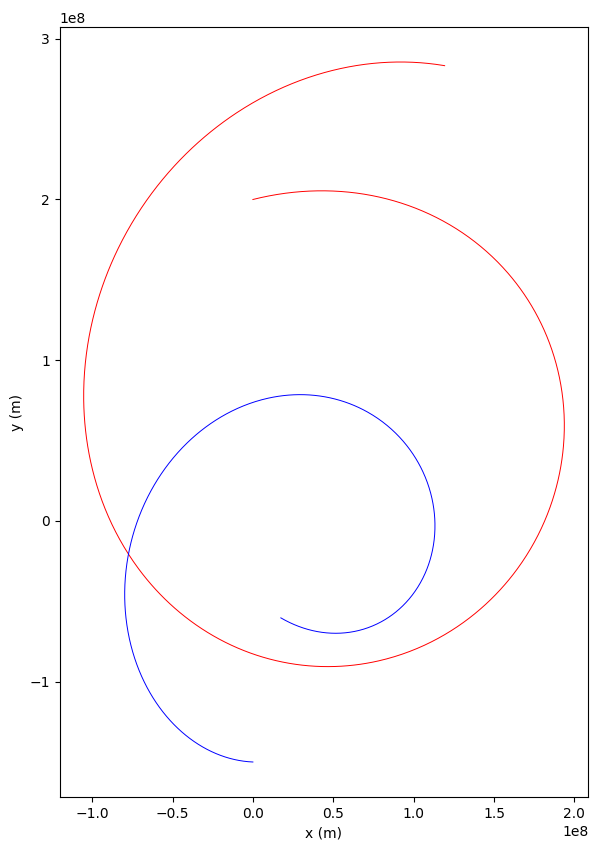
\includegraphics[width=0.5\textwidth]{plotmoons_01.png}
    \caption{Output of moons\_01.py.}
    \label{fig:plotmoons_01}
\end{figure}

It is nifty to see the paths,  but we don't know where each moon was at a particular time.  In fact, it is difficult to figure out which end of each curve was the beginning and which was the ending.

What if we added some lines and labels every 300 steps to put a sense of time into the plot?  Add one more constant after the import statements:
\begin{verbatim}
PAIR_LINE_STEP = 300  # How time steps between pair lines
\end{verbatim}


Immediately before you
save the figure to the file,  add the following code:

\begin{verbatim}
# Draw some pair lines that help the
# viewer understand time in the graph
i = 0
while i < len(positions1):

    # Where are the moons at the ith entry?
    a = positions1[i, :]
    b = positions2[i, :]
    ax.plot([a[0], b[0]], [a[1], b[1]], "--", c="gray", lw=0.6, marker=".")

    # What is the time at the ith entry?
    t = time_log[i]

    # Label the location of moon 1 with the day
    ax.text(a[0], a[1], f"{t/SEC_PER_DAY:.0f} days")
    i += PAIR_LINE_STEP
\end{verbatim}

When you run it,  your plot should look like this:
\begin{figure}[htbp]
    \centering
    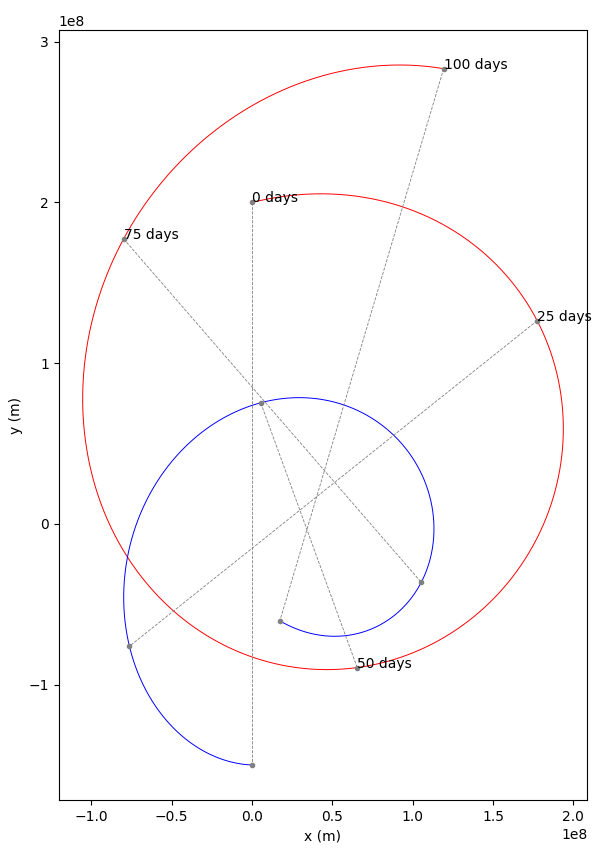
\includegraphics[width=0.5\textwidth]{plotmoons_02.png}
    \caption{Plot moons\_02.py.}
\end{figure}

Now you can get a feel for what happened.  The moons were attracted to each other by gravity and started to circle each other. The heavier moon accelerates less quickly,  so it makes a smaller loop.

Maybe we will get a better feel for what is happening if we look at more time. Let's increase it to 400 days. Change the relevant constant:

\begin{verbatim}
MAX_TIME = 400 * SEC_PER_DAY # 100 days
\end{verbatim}

Now it should look like this:
\begin{figure}[htbp]
    \centering
    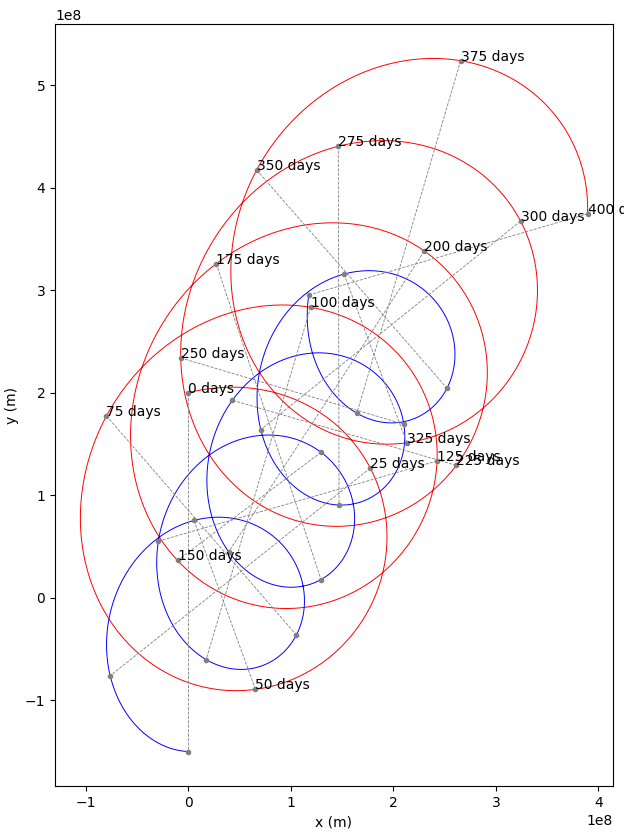
\includegraphics[width=0.5\textwidth]{plotmoons_03.png}
    \caption{Output of plot moons\_03.py.}
\end{figure}

Now you can see the pattern. They are rotating around each other and the pair is gradually migrating
up and to the right.

\section{Conservation of Momentum}
Recall the idea of momentum being conserved in a system. In these programs, you are observing an extra important idea: \emph{the momentum of a system will be conserved}. That is, absent forces from outside the system,  the velocity of the center of mass will not change.

We can compute the initial center of mass and its velocity.   In both cases,  we just do a weighted average using the mass of the moon as the weight. 

Immediately after you initialize the state of two moons,  calculate the initial center of mass and its velocity:
\begin{verbatim}
# Calculate the initial position and velocity of the center of mass
tm = m1["mass"] + m2["mass"]  # Total mass
cm_position = (m1["mass"] * m1["position"] + m2["mass"] * m2["position"]) / tm
cm_velocity = (m1["mass"] * m1["velocity"] + m2["mass"] * m2["velocity"]) / tm
\end{verbatim}

Let's record the center of mass for each time.   Before the loop starts,  create a list to hold them:

\begin{verbatim}
cm_log = []
\end{verbatim}

Inside the loop (before any calculations),  append the current center of mass position to the log:

\begin{verbatim}
    cm_log.append(cm_position)
\end{verbatim}

Anywhere later in the loop (after you update the positions of the moon),  update \pyvar{cm\_position}:

\begin{verbatim}
    # Update the center of mass
    cm_position = cm_position + cm_velocity * TIME_STEP
\end{verbatim}

Now, let's look at the positions of the moons relative to the center of mass.   Before you do any plotting,  
convert the list to a numpy array and subtract it from the positions:

\begin{verbatim}
cms = np.array(cm_log)

# Make positions relative to the center of mass
positions1 = positions1 - cms
positions2 = positions2 - cms
\end{verbatim}

When you run it, you can really see what is happening:
\begin{figure}[htbp]
    \centering
    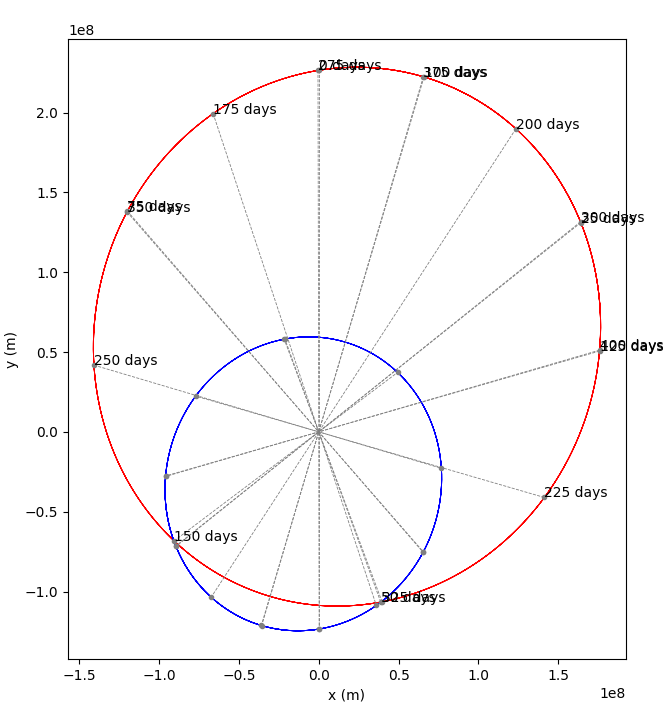
\includegraphics[width=0.5\textwidth]{plotmoons_04.png}
    \caption{Output of plotmoons\_04.py.}
    \label{fig:plotmoons_04}
\end{figure}

The moons are tracing elliptical paths.  The center of mass is the focus point for both of them.

\section{Animation}

One of the features of matplotlib that not a lot of people understand is how to make animations with it.  This
seems like a really great opportunity to make an animation showing the position, velocity, acceleration of the moons.  We will also show the center of mass.

The trick to animations is that you create a bunch "artist" objects.  You create a function that updates the 
artists. matplotlib will call your functions,  tell the artists to draw themselves,  and make a movie out of that.

Make a copy of \filename{moons.py} called \filename{animate\_moons.py}. 

Edit it to look like this:
\begin{verbatim}
import numpy as np
import matplotlib.pyplot as plt

# Import animation support and artists
from matplotlib.animation import FuncAnimation
from matplotlib.patches import Circle, FancyArrow
from matplotlib.text import Text

# Constants
G = 6.67430e-11  # Gravitational constant (Nm^2/kg^2)
SEC_PER_DAY = 24 * 60 * 60  # How many seconds in a day?
MAX_TIME = 400 * SEC_PER_DAY  # 100 days
TIME_STEP = 12 * 60 * 60  # Update every 12 hours
FRAMECOUNT = MAX_TIME / TIME_STEP  # How many frames in animation
ANI_INTERVAL = 1000 / 50  # ms for each frame in animation

# The velocity and acceleration vectors are invisible
# unless we scale them up.  A lot.
VSCALE = 140000.0
ASCALE = VSCALE * 800000.0

# Create the inital state of Moon 1
m1 = {
    "mass": 6.0e22,  # kg
    "position": np.array([0.0, 200_000_000]),  # m
    "velocity": np.array([100.0, 25.0]),  # m/s
    "radius": 1_500_000.0,  # m
    "color": "red",  # For plotting
}

# Create the inital state of Moon 2
m2 = {
    "mass": 11.0e22,  # kg
    "position": np.array([0.0, -150_000_000]),  # m
    "velocity": np.array([-45.0, 2.0]),  # m/s
    "radius": 2_000_000.0,  # m
    "color": "blue",  # For plotting
}

# Calculate the initial position and velocity of the center of mass
tm = m1["mass"] + m2["mass"]  # Total mass
cm_position = (m1["mass"] * m1["position"] + m2["mass"] * m2["position"]) / tm
cm_velocity = (m1["mass"] * m1["velocity"] + m2["mass"] * m2["velocity"]) / tm

# Start at time zero seconds
current_time = 0.0

# Create the figure and axis
fig, ax = plt.subplots(1, figsize=(7.2, 10))

# Set up the axes
ax.set_xlabel("x (m)")
ax.set_xlim((-1.2e8, 4e8))
ax.set_ylabel("y (m)")
ax.set_ylim((-1.6e8, 5.5e8))
ax.set_aspect("equal", adjustable="box")
fig.tight_layout()

# Create artists that will be edited in animation
time_text = ax.add_artist(Text(0.03, 0.95, "", transform=ax.transAxes))
circle1 = ax.add_artist(Circle((0, 0), radius=m1["radius"], color=m1["color"]))
circle2 = ax.add_artist(Circle((0, 0), radius=m2["radius"], color=m2["color"]))
circle_cm = ax.add_artist(Circle((0, 0), radius=m2["radius"], color="purple"))
varrow1 = ax.add_artist(FancyArrow(0, 0, 0, 0, color="green", head_width=m1["radius"]))
varrow2 = ax.add_artist(FancyArrow(0, 0, 0, 0, color="green", head_width=m2["radius"]))
acc_arrow1 = ax.add_artist(
    FancyArrow(0, 0, 0, 0, color="purple", head_width=m1["radius"])
)
acc_arrow2 = ax.add_artist(
    FancyArrow(0, 0, 0, 0, color="purple", head_width=m2["radius"])
)


# This function will get called for every frame
def animate(frame):

    # Global variables needed in scope from the model
    global cm_position, cm_velocity, current_time, m1, m2

    # Global variables needed in scope from the artists
    global time_text, varrow1, varrow2, acc_arrow1, acc_arrow2, circle1, circle2, circle_cm

    print(f"Updating artists for day {current_time/SEC_PER_DAY:.1f}.")

    # Update the positions based on the current velocities
    m1["position"] = m1["position"] + m1["velocity"] * TIME_STEP
    m2["position"] = m2["position"] + m2["velocity"] * TIME_STEP

    # Update day label
    time_text.set_text(f"Day {current_time/SEC_PER_DAY:.0f}")

    # Update positions of circles
    circle1.set_center(m1["position"])
    circle2.set_center(m2["position"])

    # Update velocity arrows
    varrow1.set_data(
        x=m1["position"][0],
        y=m1["position"][1],
        dx=VSCALE * m1["velocity"][0],
        dy=VSCALE * m1["velocity"][1],
    )
    varrow2.set_data(
        x=m2["position"][0],
        y=m2["position"][1],
        dx=VSCALE * m2["velocity"][0],
        dy=VSCALE * m2["velocity"][1],
    )

    # Update the center of mass
    cm_position = cm_position + cm_velocity * TIME_STEP
    circle_cm.set_center(cm_position)

    # Find the vector from moon1 to moon2
    delta = m2["position"] - m1["position"]

    # What is the distance between the moons?
    distance = np.linalg.norm(delta)

    # Have the moons collided?
    if distance < m1["radius"] + m2["radius"]:
        print(f"*** Collided {current_time:.1f} seconds in!")

    # What is a unit vector that points from moon1 toward moon2?
    direction = delta / distance

    # Calculate the magnitude of the gravitational attraction
    magnitude = G * m1["mass"] * m2["mass"] / (distance**2)

    # Acceleration vector of moons (a = f/m)
    acceleration1 = direction * magnitude / m1["mass"]
    acceleration2 = (-1 * direction) * magnitude / m2["mass"]

    # Update the acceleration arrows
    acc_arrow1.set_data(
        x=m1["position"][0],
        y=m1["position"][1],
        dx=ASCALE * acceleration1[0],
        dy=ASCALE * acceleration1[1],
    )
    acc_arrow2.set_data(
        x=m2["position"][0],
        y=m2["position"][1],
        dx=ASCALE * acceleration2[0],
        dy=ASCALE * acceleration2[1],
    )

    # Update the velocity vectors
    m1["velocity"] = m1["velocity"] + acceleration1 * TIME_STEP
    m2["velocity"] = m2["velocity"] + acceleration2 * TIME_STEP

    # Update the clock
    current_time += TIME_STEP

    # Return the artists that need to be redrawn
    return (
        time_text,
        varrow1,
        varrow2,
        acc_arrow1,
        acc_arrow2,
        circle1,
        circle2,
        circle_cm,
    )


# Make the rendering happen
animation = FuncAnimation(
    fig, 
    animate, 
    np.arange(FRAMECOUNT), 
    interval=ANI_INTERVAL
)

# Save the rendering to a video file
animation.save("moonmovie.mp4")
\end{verbatim}

When you run this,  it will take longer than the previous versions.  You should have a 
video file that shows a simulation of the moons tracing their elliptical paths around their
center of mass:
\begin{figure}[htbp]
    \centering
    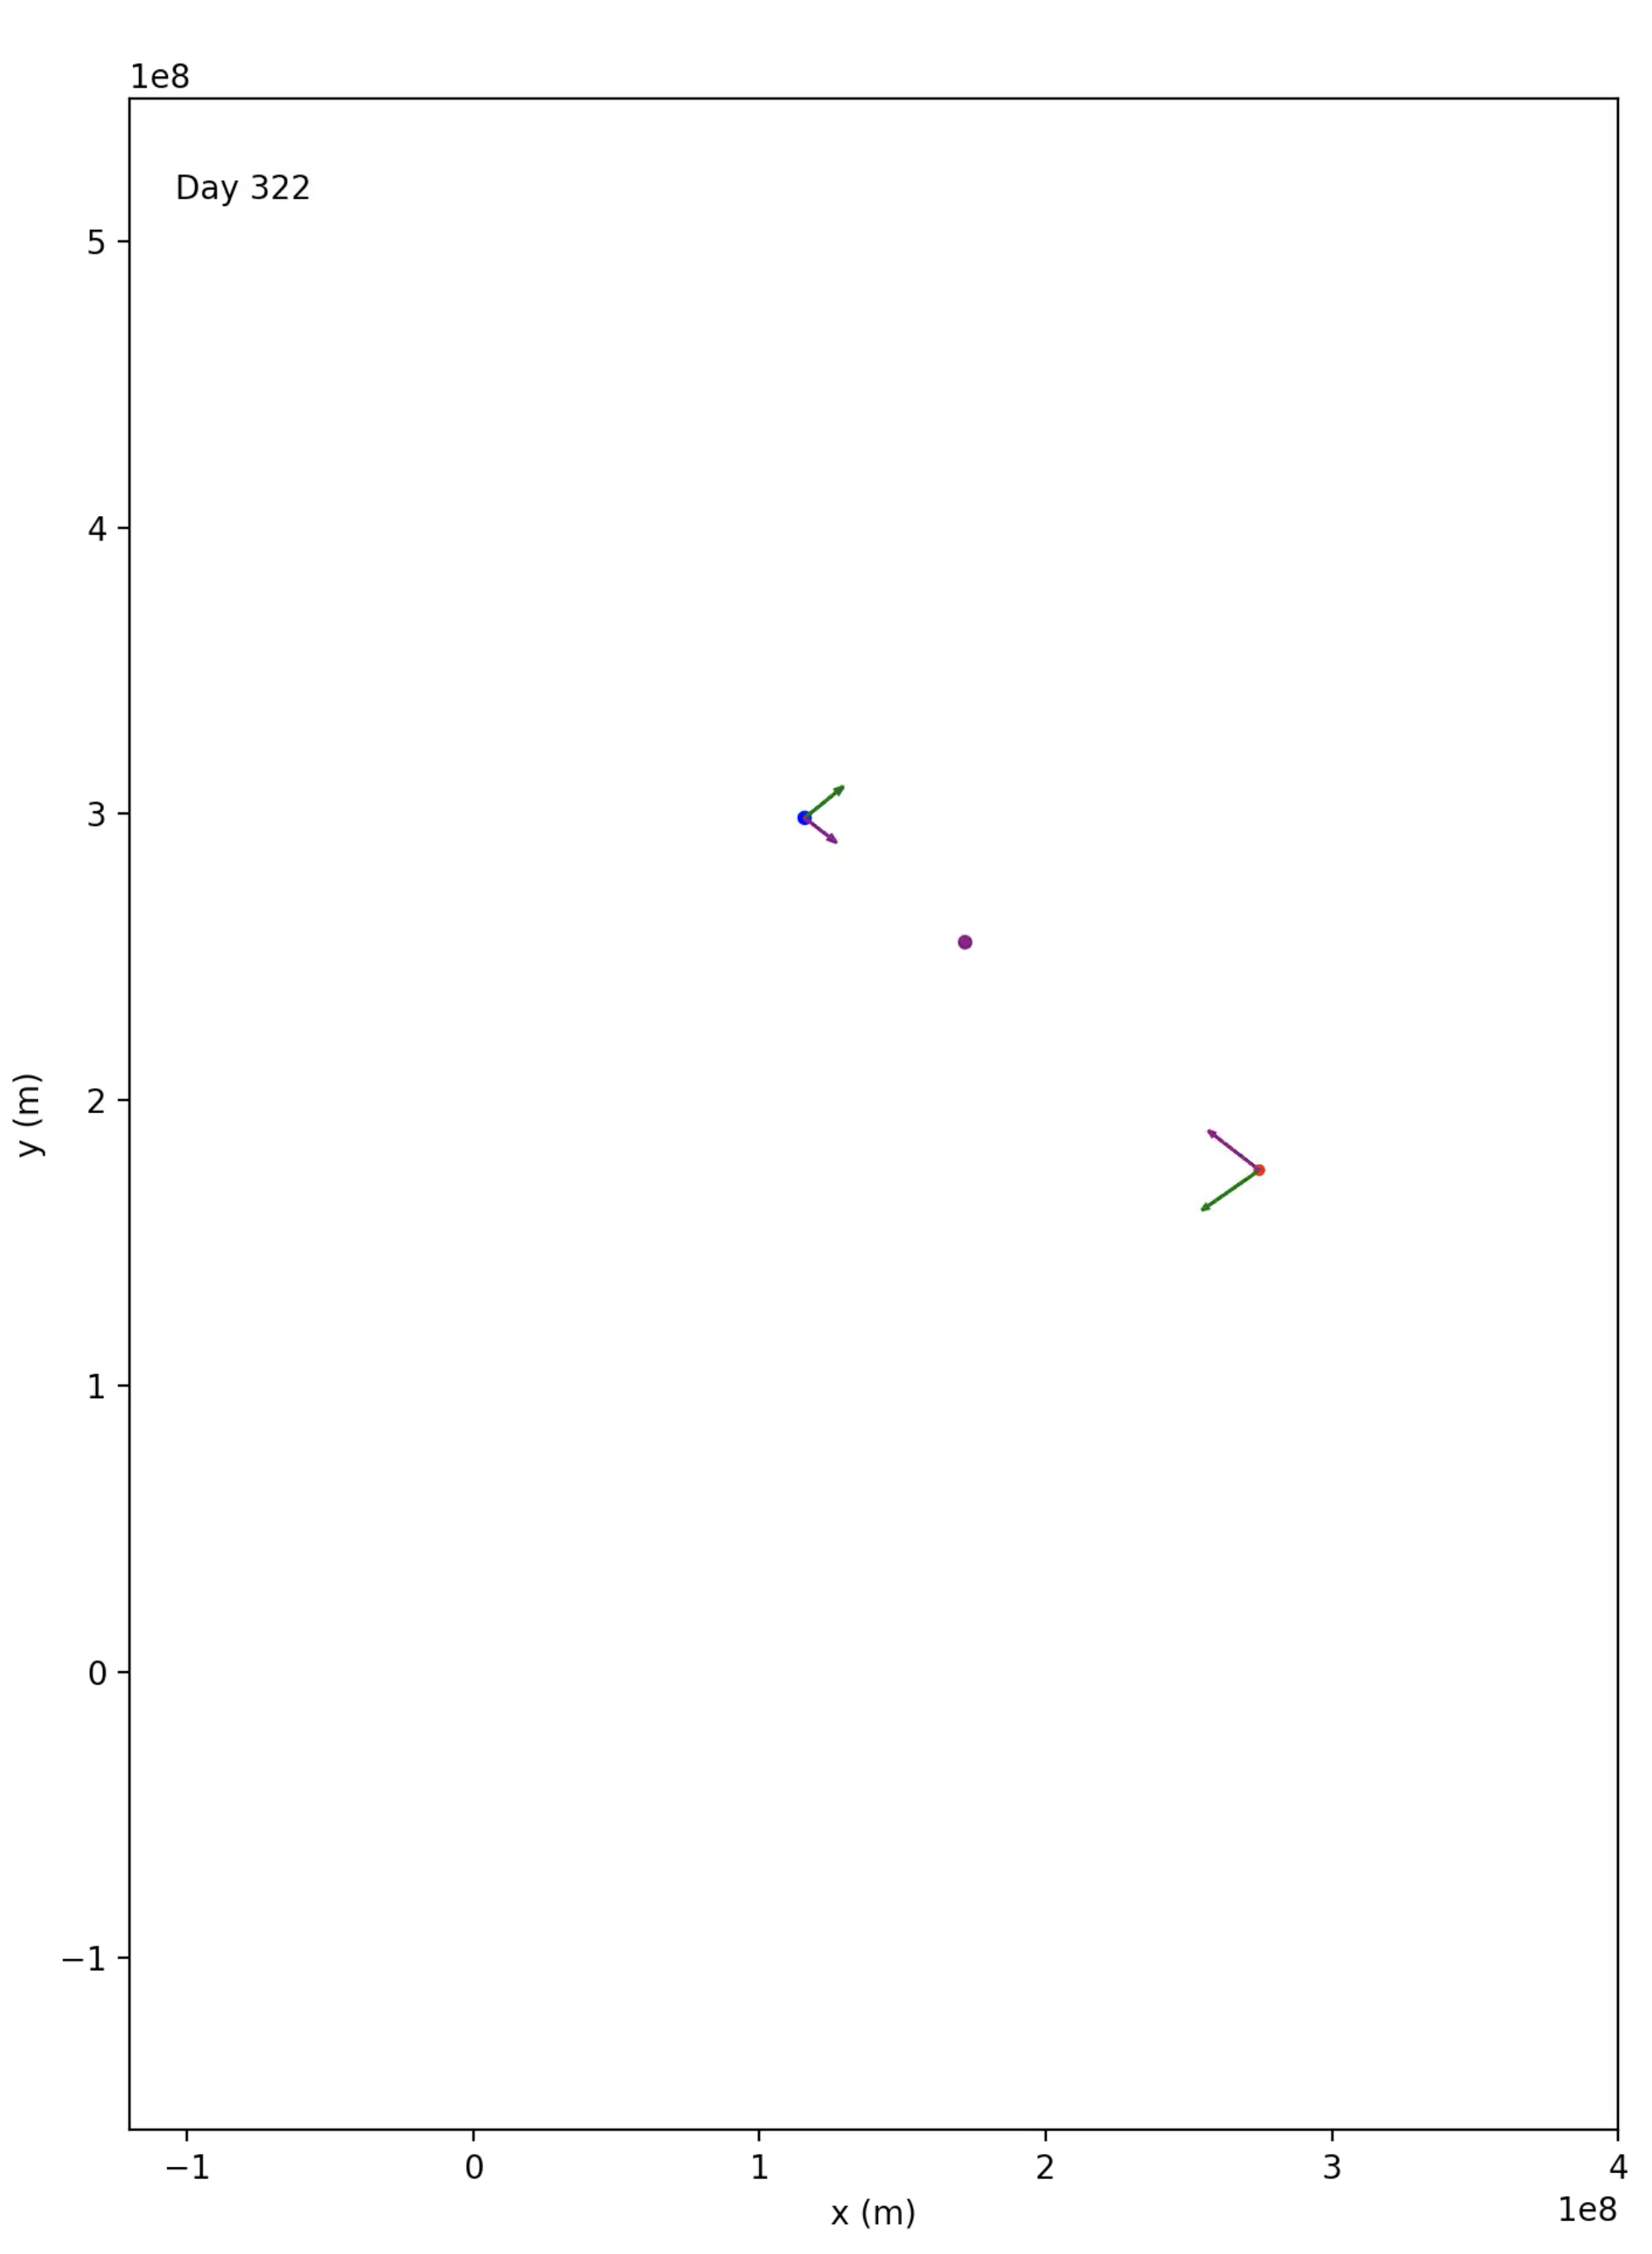
\includegraphics[width=0.5\textwidth]{movie.png}
    \caption{A still of the animation produced.}
    \label{fig:movie}
\end{figure}

\section{Challenge: The Three-Body Problem}
\index{Three-Body Problem}
It is time to stretch a little as a physicist and programmer:  You are going to make a new version of \filename{moons.py} that handles three moons instead of just two.

This is known as ''The Three-Body Problem'', and people have tried for centuries to come up with 
a way to figure out (from the initial conditions) where the three moons would be at time $t$ without doing a simulation.  And no one has.

For a lot of problems,  the outcome is not very sensitive to the initial conditions. For example, consider the flight of a
cannonball:  If it leaves the muzzle of the cannon a little faster,  it will go a little farther.

For the three-body problem,  the outcome can be radically different even if the initial conditions are very similar.  

(There is a whole field of mathematics studying systems that are very sensitive to initial conditions.  It is known
as \newterm{dynamical systems} or \newterm{chaos theory}.)

Copy \filename{moons.py}  to \filename{3moons.py}.  Here is a reasonable initial state for your third moon:

\begin{verbatim}
m3 = {
    "mass": 4.0e22,  # kg
    "position": np.array([50_000_000, 80_000_000]),  # m
    "velocity": np.array([-30.0, -35.0]),  # m/s
    "radius": 1_700_000.0,  # m
    "color": "green" 
}  
\end{verbatim}

If we run that simulation for 100 days, we get a plot like this:
\begin{figure}[htbp]
    \centering
    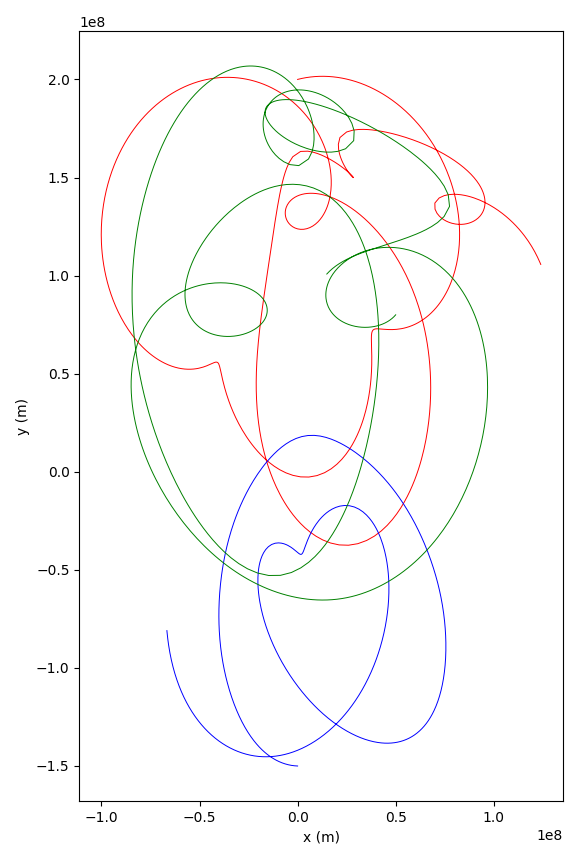
\includegraphics[width=0.6\textwidth]{plot3moons_01.png}
    \caption{The Three Body Problem.}
    \label{fig:threebodyproblem}
\end{figure}

Visibly, you can see this is very different from the two-body problem that just traced ellipses around the center of mass.
